\subsection{Scheduling object construction}
\label{sec:architecture}
Reconstructing more objects creates more opportunities to work in parallel.
Two workers can build a desk and a chair independently. A third worker placing
a lamp on the desk needs its final height. We implement two controllers for
AHa-3D that use these dependencies while retaining its camera estimates,
geometry tools and scene review (Figure~\ref{fig:blueprint}).

\begin{figure}[!htbp]
\centering
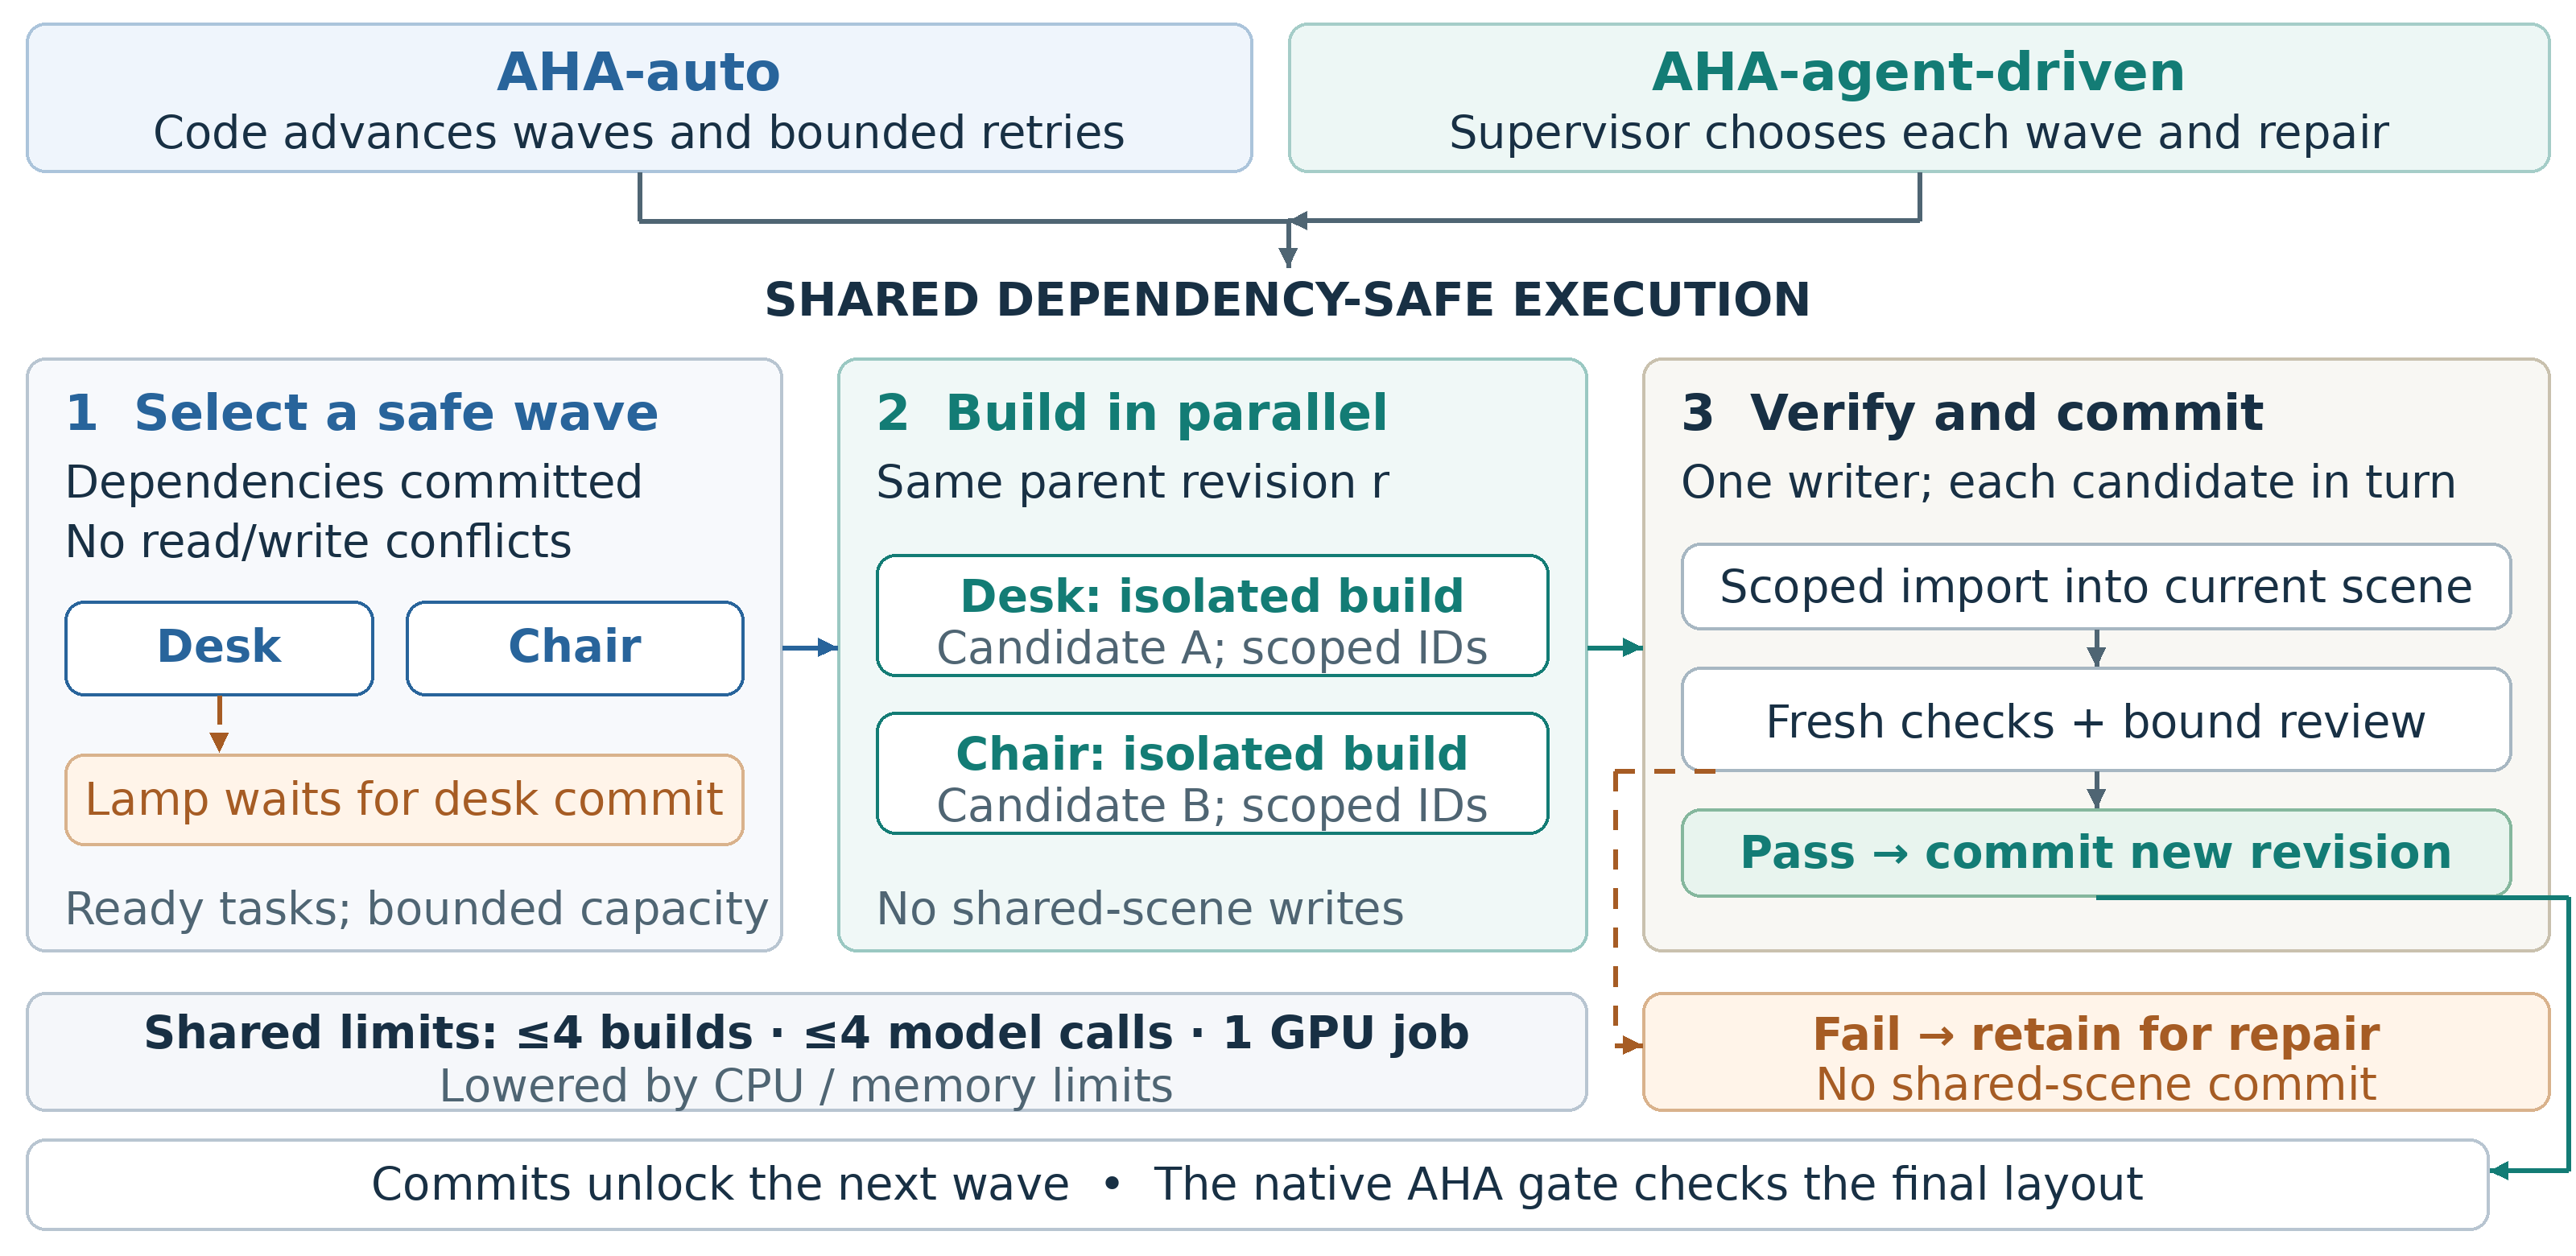
\includegraphics[width=\linewidth]{figures/parallelism.png}
\caption{The desk and chair can be built from the same scene. The lamp waits
for the desk to be committed. Workers build isolated candidates, and a single
writer incorporates reviewed edits into the shared room.}
\label{fig:blueprint}
\end{figure}

In \textbf{AHA-auto}, a model plans the tasks and a program dispatches ready
work, retries failed builds and escalates difficult cases to a stronger model.
In \textbf{AHA-agent-driven}, a supervisor chooses which tasks to delegate,
when to review them and how to repair a failed edit. Both controllers allow
tasks to run together only after their prerequisites are complete and when
neither task changes objects the other uses.

Workers edit separate scene copies. Before an edit becomes part of the room,
the controller checks the saved geometry and cameras, verifies that unrelated
objects were preserved and reviews the proposed change against the current
scene. A short Blender benchmark and available memory limit the number of
simultaneous builds. GPU generation and writes to the shared scene run serially.
